\subsection{Lecture 24}
\subsubsection{Geometry of LLSE}

We can always think of the LLSE $L[X \mid Y]$ as the projection of $X$ onto the subspace $\mathcal{L}(Y)$ of linear functions of $Y$.
To do this, first we have to set up the idea of a Hilbert space.

\begin{definition}[Vector Space]
    A set $S$ is a vector space if it's closed under addition and scalar multiplication (among other properties).
\end{definition}

\begin{definition}[Hilbert Space]
    A set $\mathcal{H}$ is a Hilbert space if it's a vector space that has an inner product and is complete (all limits of convergent sequences are in the space).
\end{definition}

\begin{definition}[Inner Product]
    An (real) inner product on a vector space $S$ is an operation $\langle \cdot, \cdot \rangle : S \to \R$
    that satisfies.
\end{definition}

\begin{definition}[Norm]
    The norm or length of a vector $v$ given an inner product is $\norm{v} = \sqrt{\langle v, v \rangle}$.
\end{definition}

We now extend our optimization-motivated LLSE in order to allow our estimate to be a general function, i.e. the MMSE. First, we claim that
the LLSE $L[X \mid Y]$ is the "projection" of $X$ onto the subspace of affine functions of $Y$, i.e. $\mathcal{L}(Y) = \{ c + dY \mid c, d \in \R \}$. This is a vector space,
but we need an inner product to make it a Hilbert space. For any space of RVs, let us define the inner product as:
\[ \langle V, W \rangle = \E{VW} \]
We define orthogonality based on if the inner product is 0, i.e. two random variables $V$ and $W$ are orthogonal if $\E{VW} = 0$.

\begin{theorem}[Hilbert's Projection Theorem]
    Consider some Hilbert space $\mathcal{H}$ and $a \in \mathcal{H}$ and some subspace $U$ of $\mathcal{H}$. Then, there exists a linear projection operator $P$ that projects onto $U$
    (finds the element of $U$, $u^*$, such that $||a - u^*||$ is minimized),
    so the projection of is $Pa$. Then, we claim that the error, $a - Pa \in U^{\perp}$, i.e. for any $u \in U$, $\langle a - Pa, u \rangle = 0$.
\end{theorem}

In particular, our claim of LLSE projection can be rewritten as:

\begin{theorem}[Projection Property]
    $X - L[X \mid Y] \in \mathcal{L}(Y)^{\perp}$, where $Z^\perp$ denotes the orthogonal complement to vector space $Z$. In particular, this means it is orthogonal
    to every affine function of $Y$.

    \begin{proof*}
        Call $L[X \mid Y] = a + bY$. Consider $c + dY \in \mathcal{L}(Y)$. Then, we will show $\E{(X - a - bY)(c + dY)} = 0$.
        We know from our partial derivatives before, in the proof of Theorem 7.1,
        \begin{align*}
            \E{X - a - bY} &= 0 \\
            \E{Y(X - a - bY)} &= 0
        \end{align*}
        Thus, taking $c$ times the the first equation and adding $d$ times the second equation shows the claim.
    \end{proof*}
\end{theorem}


This implies, from the Hilbert Projection Theorem, that $L[X \mid Y]$ is the closest point to $X$ in $\mathcal{L}(Y)$. However, we can prove this
without invoking the result.

\begin{proof*}
    We will show $\E{(X - L[X \mid Y])^2} \leq \E{(X - h(Y))^2}$ for any $h(Y) = c + dY$. To do this, note that:
    \begin{align*}
        \E{(X - h(Y))^2} &= \E{(X - L[X\mid Y] + L[X \mid Y] - h(Y))^2} \\
        &= \E{(X - L[X \mid Y])^2} + \E{(L[X \mid Y] - h(Y))^2} + 2 \E{(X - L[X \mid Y])(L[X \mid Y] - h(Y))}
    \end{align*}
    Note that $L[X \mid Y] - h(Y) \in \mathcal{L}(Y)$, so it must be orthogonal to the error. This means the cross term is 0. This yields:
    \[ \E{(X - h(Y))^2} \geq \E{(X - L[X \mid Y])^2} \]
    with equality if the other square term is 0, i.e. $h(Y) = L[X \mid Y]$.
\end{proof*}

Now remember our online/offline regression problem; we can replace all the statistics by their sample estimates (like sample average). By law of large numbers,
as the number of samples increases, the linear regression approaches the LLSE estimate.

\subsubsection{MMSE}

We now consider the MMSE problem. We want to find the function $g$ such that $g(Y)$ minimizes $\E{(X - g(Y))^2}$.

\begin{theorem}[MMSE]
    MMSE of $X$ given $Y$ is given by $g(Y) = \E{X \mid Y}$.
\end{theorem}

Remember that $\E{X \mid Y}$ is a random variable, and $\E{X \mid Y = y} = \int_{-\infty}^{\infty} x f_{X \mid Y}(x \mid y) \dd{x}$
where $f_{X \mid Y} (x \mid y) = \frac{f_{X, Y}(x, y)}{f_Y(y)}$.

\begin{theorem}[Orthogonality of MMSE]
    \begin{itemize}
        \item For any function $\phi(\cdot)$, $\E{(X - \E{X \mid Y}) \phi(Y)} = 0$. 
        \item If $g(Y)$ is such that $X - g(Y)$ is orthogonal to any function of $Y$, $g(Y) = \E{X \mid Y}$ (i.e. it's the unique function with this property).
    \end{itemize}

    \begin{proof*}
        We start with the first claim. Consider the following tower rule expression with arbitrary $\phi(Y)$:
        \begin{align*}
            \E{\E{X \mid Y} \phi(Y)} &= \int_{-\infty}^{\infty} \E{X \mid Y = y} \phi(y) f_Y(y) \dd{y} \\
            &= \int_{-\infty}^{\infty} \int_{-\infty}^{\infty} x \frac{f_{X, Y}(x, y)}{f_Y(y)} \phi(y) f_Y(y) \dd{x} \dd{y} \\
            &= \int_{-\infty}^{\infty} \int_{-\infty}^{\infty} x \phi f_{X, Y}(x, y) \dd{x} \dd{y} \\
            &= \E{x \phi(y)}
        \end{align*}
        Thus, this means that $\E{X \phi(Y) - \E{X \mid Y} \phi(Y)} = 0$, as we wanted to show.

        The second claim is that of uniqueness. Consider some $g(Y)$ which has $X - g(Y)$ orthogonal to any function of $Y$. We will show the norm of $g(Y) - \E{X \mid Y}$ is $0$, meaning they must be the same random variable almost surely.
        \begin{align*}
            \E{(g(Y) - \E{X \mid Y})^2} &= \E{(g(Y) - \E{X \mid Y})((g(Y) - X) - (\E{X \mid Y} - X))} \\
            &= \E{(g(Y) - \E{X \mid Y})((g(Y) - X)} - \E{(g(Y) - \E{X \mid Y})(\E{X \mid Y} - X)}
        \end{align*}
        Call the first term $T_1$, the second term $T_2$. $\E{T_1} = 0$ because its left term is a function of $Y$ and $g(Y) - X$ is error, so they must be orthogonal.
        Furthermore, $\E{T_2} = 0$ because its left term is a function of $Y$ and $\E{X \mid Y} - X$ is error, so they must be orthogonal.
    \end{proof*}
\end{theorem}

By the Hilbert projection theorem, this theorem shows the form of the MMSE as $\E{X \mid Y}$. You can prove this similarly to the LLSE case using the
Pythagorean Theorem.

Here is a lot of properties of conditional expectation.

\begin{theorem}[Properties of MMSE]
    \begin{itemize}
        \item Linearity: $\E{a_1 X_1 + a_2 X_2 \mid Y} = a_1 \E{X_1 \mid Y} + a_2 \E{X_2 \mid Y}$
        \item Factoring: $\E{h(Y) X \mid Y} = h(Y) \E{X \mid Y}$
        \item Independence: If $X$ and $Y$ are independent, $\E{X \mid Y} = \E{X}$
        \item Smoothing: $\E{\E{X \mid Y}} = \E{X}$
        \item Tower: $\E{\E{X \mid Y, Z} \mid Y} = \E{X \mid Y}$
    \end{itemize}
    Let's prove the last of them, which the most tricky of the bunch.

    \begin{proof*}
        Let $\E{X \mid Y, Z} = R$, where $R \in \mathcal{G}(Y, Z)$. We want to show the error of the estimation is 0.
        \begin{align*}
            \E{(R - \E{X \mid Y}) \phi(Y)} &= \E{(X - \E{X \mid Y}) \phi(Y)} - \E{(X - R) \phi(Y)} \\
        \end{align*}
        Clearly the first term is 0 from our orthogonality lemma. Note that $X - R$ is the error from $\E{X \mid Y, Z}$,
        but $\phi(Y) \in \mathcal{G}(Y) \subseteq \mathcal{G}(Y, Z)$, so the second term is also 0. This means that the error is indeed 0,
        meaning that $R - \E{X \mid Y}$ is orthogonal to $Y$. meaning that $\E{R \mid Y} = \E{X \mid Y}$.
    \end{proof*}
\end{theorem}

Let us do some examples to practice the properties.

\begin{example}
    Let $X, Y$ be IID $U[0, 1]$. We wish to find $\E{(X + 2Y)^2 \mid Y}$.
    \begin{align*}
        \E{(X + 2Y)^2 \mid Y} &= \E{X^2 \mid Y} + 4 \E{Y^2 \mid Y} + 4 \E{XY \mid Y} \\
        &= \E{X^2} + 4Y^2 + 4Y\E{X} \\
        &= 4Y^2 + 2Y + \frac13
    \end{align*}
\end{example}

\begin{example}
    Let $X, Y, Z$ be IID. We want to compute $e = \E{X \mid X + Y + Z}$. Notice by symmetry,
    \[ e = \E{Y \mid X + Y + Z} = \E{Z \mid X + Y + Z} \]
    This means that $\E{(X + Y+ Z) \mid (X + Y + Z)} = 3e$. Thus, $3e = (X + Y + Z)$.
    Our answer is $e = \frac{X + Y+ Z}{3}$.
\end{example}

Returning to our Jointly-Gaussian RVs, we have an even cleaner result.

\begin{theorem}
    Let $X, Y$ be JG RVs. Then,
    \[ \E{X \mid Y} = L{X \mid Y} = \E{X} + \frac{\Cov{X, Y}}{\Var{Y}} ( Y- \E{Y}) \]

    \begin{proof*}
        We first note that $X - L[X \mid Y]$ and $Y$ are uncorrelated, because:
        \begin{align*}
            \Cov(X - L[X \mid Y], Y) &= \E{(X - L[X \mid Y]) Y} - \E{X - L[X \mid Y]} \E{Y} \\
            &= 0 - (\E{X} - \E{\E{X} + \frac{\Cov{X, Y}}{\Var{Y}}(Y - \E{Y})}) \E{Y} \\
            &= 0 \cdot \E{Y} = 0
        \end{align*}

        Also, then $X - L[X \mid Y]$ and $Y$ are JG, as they are linear combinations of $X$ and $Y$. This means that $X - L[X \mid Y]$ and $Y$ are independent.
        This means that:
        \begin{align*}
            \E{X - L[X \mid Y] \mid Y} &= \E{X - L[X \mid Y]} \\
            &= 0
            \E{X \mid Y} &= \E{L[X \mid Y] \mid Y} \\
            &= L[X \mid Y]
        \end{align*}
    \end{proof*}
\end{theorem}

We also have the following properties of LLSE.
\begin{theorem}
    The LLSE $L[\cdot \mid \cdot]$ satisfies:
    \begin{enumerate}
        \item $L[a_1 X_1 + a_2 X_2 \mid Y] = a_1 L[X_1 \mid Y] + a_2 L[X_2 \mid Y]$.
        \item $L[L[X \mid Y, Z] \mid Y] = L[X \mid Y]$.
        \item If $X, Y$ are uncorrelated, $L[X \mid Y] = \E{X}$.
    \end{enumerate}
    \begin{proof*}
        We will show the second property (the rest are not too bad). Consider the error vector of the LHS:
        $L[X \mid Y, Z] - L[X \mid Y]$; we will show it is orthogonal to $Y$. Adding and subtracting $X$ gives:
        $-(X - L[X \mid Y, Z]) + (X - L[X \mid Y])$. Both terms are orthogonal to 1, $Y$, so the error vector is orthogonal to 1, $Y$.
        This means that it is the LLSE, as we wanted to show.
    \end{proof*}
\end{theorem}

Lastly, we have a few results for LLSE that can be explained mostly geometrically.

\begin{theorem} [LLSE Orthogonal Update]
    Assume that $X, Y, Z$ are zero-mean random variables, and that $Y, Z$ are orthogonal. Then, $L[X \mid Y, Z] = L[X \mid Y] + L[X \mid Z]$.
    \begin{proof*}
        To show this result, we need to show the projection error is orthogonal to $Y$ and $Z$ (because then it would be orthogonal to any linear combination there of).
        The error is $X - (L[X \mid Y] + L[X \mid Z])$. The first two terms together are orthogonal to $Y$, and the last term is linear in $Z$, so it is also orthogonal to $Y$.
        By a similar argument, the expression is orthogonal to $Z$. Thus, we are done, and this is uniquely the LLSE.
    \end{proof*}
\end{theorem}

You can see this alternatively by looking at the following diagram:

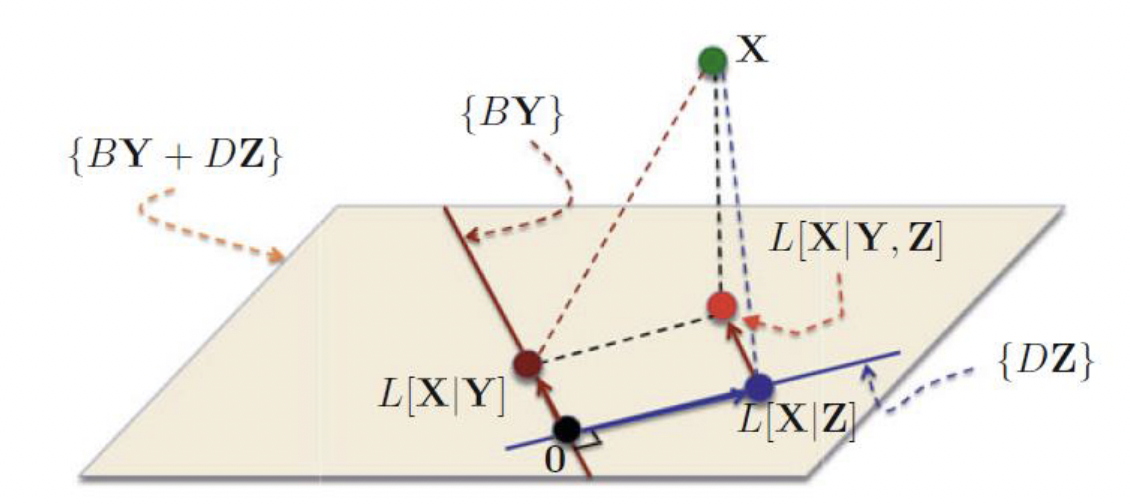
\includegraphics[width=300px]{orthogonal_update.png}

We can project onto the subspaces separately and then add them up. Note that the projection error is smaller than the projection on either of the subspaces individually (this is intuitively appealing).

\begin{theorem}[LLSE General Update]
    Assume that $X, Y, Z$ are zero-mean random variables. Then, $L[X \mid Y, Z] = L[X \mid Y] + L[X \mid Z -  L[Z \mid Y]]$.
    \begin{proof*}
        Let $\tilde{Z} = Z - L[Z \mid Y]$.
        We know $\tilde{Z} \perp Y$, and furthermore any linear combination of $Y, Z$ can be turned into a linear combination of $Y, \tilde{Z}$ (Suppose $L[Z \mid Y] = cY$ to see this).
        Thus, this means that $L[X \mid Y, Z] = L[X \mid Y, \tilde{Z}] = L[X \mid Y] + L[X \mid \tilde{Z}]$ as we wanted to show.
    \end{proof*}
\end{theorem}

We consider the term $\tilde{Z}$ as the "innovation" i.e. the new information we glean from new observation $Z$.
